\documentclass[addpoints,12pt]{exam}
\usepackage{amsmath}
\usepackage{amsthm}
\usepackage{amsfonts}
\usepackage{systeme}
\usepackage{graphicx}
\usepackage{caption}
\usepackage{xfrac}
\usepackage{physics}
\usepackage{microtype}
\usepackage{eulervm}
%\usepackage[framemethod=tikz]{mdframed}
\usepackage{thmtools}
\usepackage{etoolbox}
%\usepackage{fouriernc}
\usepackage{mdframed}
\usepackage[overload]{empheq}
\usepackage{adjustbox}
\usepackage{enumitem}
\usepackage[explicit]{titlesec}
% adds in \varnothing for empty set
\usepackage{amssymb}
% adds in formated SI units
%\usepackage{siunitx}

\pagestyle{headandfoot}
\runningfootrule
\firstpageheadrule
\runningheadrule

\newcommand{\class}{Math 0097}
\newcommand{\sem}{2211}
\newcommand{\due}{}
\newcommand{\sect}{2.6}
\newcommand{\topic}{Problem Solving with Geometry}

\firstpageheader{\class}{\sect - \topic}{}
\runningheader{\class}{\sect - \topic}{}
\firstpagefooter{\class}{}{Page \thepage\ of \numpages}
\runningfooter{\class}{}{Page \thepage\ of \numpages}

\newif\ifprintselected
\printselectedtrue
%\printselectedfalse

\newenvironment{select}
{\ifprintselected
	\printanswers
	\fi
}
{}

\theoremstyle{definition}
\newtheorem{theorem}{Theorem}
%\newtheorem{example}{Example}[subsection]
%\newtheorem{definition}{Definition}
%\newmdtheoremenv{definition}{Definition}[subsection]
%\newmdtheoremenv{example}{Example}[subsection]
\AtBeginEnvironment{defn}{\begin{minipage}{\textwidth}}
\AtEndEnvironment{defn}{\end{minipage}}
%\AtBeginEnvironment{example}{\begin{minipage}{\textwidth}}
%\AtEndEnvironment{example}{\end{minipage}}
\newcommand{\iu}{{i\mkern1mu}}

\setlength{\gridsize}{5mm}
\setlength{\gridlinewidth}{0.1pt}

\printanswers
\DeclareMathSizes{12}{12}{12}{12}

%%%%%%%%%%%%%%%%%%%%%%%%
% Create bars around subsubsection
%%%%%%%%%%%%%%%%%%%%%%%%

\titleformat{\subsubsection}
   {\large\bfseries}% format
   {}% label
   {0pt}% sep
   {\titlerule \vspace{.1in} #1}% before code
      [{\titlerule[0.4pt]\vspace{.1in}}]% after code
\titlespacing{\subsubsection}
   {0pt}% left
   {0pt}% before sep
   {\baselineskip}% after sep
   
%%%%%%%%%%%%%%%%%%%%%%%
% Create line break after definition label
%%%%%%%%%%%%%%%%%%%%%%%   
\newtheoremstyle{break}
  {\topsep}{\topsep}%
  {}{}%\itshape
  {\bfseries}{}%
  {\newline}{}%
\theoremstyle{break}
\newmdtheoremenv{definition}{Definition}[subsection]
\theoremstyle{break}
\newtheorem{example}{Example}[subsection]

%%%%%%%%%%%%%%%%%%%%%%
% start document
% set section, subsection (use n-1 for sub)
%%%%%%%%%%%%%%%%%%%%%%


\begin{document}
\setcounter{section}{2}
\setcounter{subsection}{5}

\subsection{Problem Solving with Geometry}

\vspace{.25in}

\begin{definition}[Area]
the amount of 2-dimensional space that an object takes up; has square units: $ft^2,\; m^2,\; yd^2$, etc.
\end{definition}

\vspace{.15in}

\begin{definition}[Perimeter]
the length of the exterior of an objects; has linear units; found by adding the sides of a polygon
\end{definition}

\vspace{.15in}

\noindent Below are common formulas that will be used throughout this class.
\begin{figure}[h]
\centering
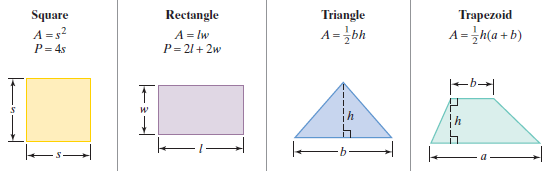
\includegraphics[scale=1]{../images/polygon_formulas}
\end{figure}
\begin{figure}[h]
\centering
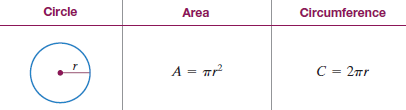
\includegraphics[scale=1]{../images/circle_formulas}
\end{figure}

\newpage

\begin{example}
Find the height of a triangular sail that has an area of 24 square feet and a base of 4 feet.
\vspace{2.5in}
\end{example}

\begin{example}
The diameter of a circular pool is 40 feet. Find the area and circumference rounded to the nearest foot.
\end{example}

\newpage

\begin{definition}[Volume]
the amount of 3-dimensional space that an object takes up; has cubic units ($m^3, ft^3, yd^3$, etc.)
\end{definition}
\vspace{.15in}

\begin{mdframed}
\textbf{Common Volume Formulas}
\begin{itemize}
\item Cube: $V = s^3$
\item Rectangular Solid: $V = lwh$
\item Cylinder: $V = \pi r^2h$
\item Sphere: $V = \dfrac{4}{3}\pi r^3$
\item Cone: $V = \dfrac{1}{3}\pi r^2h$
\end{itemize}
\end{mdframed}

\vspace{.15in}
\begin{example}
A cylinder with a radius of 3 inches and a height of 5 inches has its height doubled. How many times greater is the new volume over the old one?
\end{example}

\end{document}